\documentclass[12pt, titlepage]{article}

\usepackage{fullpage}
\usepackage[round]{natbib}
\usepackage{multirow}
\usepackage[shortlabels]{enumitem}
\usepackage{comment}
\usepackage{booktabs}
\usepackage{tabularx}
\usepackage{graphicx}
\usepackage{float}
\usepackage{hyperref}
\usepackage{pdfpages}
\usepackage{pdflscape}

\usepackage{float}
\usepackage{soul}
\usepackage{changepage}
\usepackage{graphicx}
\hypersetup{
    colorlinks,
    citecolor=black,
    filecolor=black,
    linkcolor=red,
    urlcolor=blue
}
\usepackage[round]{natbib}
\usepackage{multirow}

\input{../Comments}
%% Common Parts

\newcommand{\progname}{Measuring Microstructure Changes During Thermal Treatment} % PUT YOUR PROGRAM NAME HERE
\newcommand{\authname}{Team \#30, ReSprint
\\ Edwin Do
\\ Joseph Braun
\\ Timothy Chen
\\ Abdul Nour Seddiki
\\ Tyler Magarelli
} % AUTHOR NAMES                  

\usepackage{hyperref}
    \hypersetup{colorlinks=true, linkcolor=blue, citecolor=blue, filecolor=blue,
                urlcolor=blue, unicode=false}
    \urlstyle{same}
                                


\begin{document}

\title{Verification and Validation Report: \progname} 
\author{\authname}
\date{\today}
	
\maketitle

\pagenumbering{roman}

\section{Revision History}


\begin{tabularx}{\textwidth}{p{3cm}p{3cm}X}
\toprule {\bf Date} & {\bf Developer} & {\bf Change}\\
\midrule
Mar 7, 2023 & Abdul Nour & Updated template\\
Mar 8 2023 & Edwin Do & Added usability test results \\
Mar 8 2023 & Edwin Do & Added Traceability matrices \\
Mar 8, 2023 & Timothy Chen & Added performance to the Nonfunctional Test Evaluation\\
Mar 8, 2023 & Timothy Chen & Added unit test for input communication, current state and remote access\\
Mar 8, 2023 & Joseph Braun & Added Sections 5, 7, 8 \\
Mar 8, 2023 & Joseph Braun & Added Reflection \\
Mar 8, 2023 & Timothy Chen & Added Trace to Modules \\
Mar 8, 2023 & Abdul Nour & Added Functional Requirements Evaluation \& Trace to Requirements\\
Mar 8, 2023 & Abdul Nour & Added Functional Req's Unit Tests\\
\bottomrule
\end{tabularx}

~\newpage

\section{Symbols, Abbreviations and Acronyms}
change capacity to size

\renewcommand{\arraystretch}{1.2}
\begin{tabular}{l l} 
  \toprule		
  \textbf{symbol} & \textbf{description}\\
  \midrule 
  T & Test\\
  MIN\_USER\_ACCEPT\_RATE & 90\% - minimum acceptance rate\\
  TARGET\_TIME & 60 seconds \\
  INTERACT\_TIME & 5 seconds \\
  MAX\_MISTAKE & 2 \\
  MAX\_SIZE & 8GB \\ 
  MIN\_UPTIME & 30 minutes \\ 
  MIN\_SAMPLE\_RATE & 60 samples per second\\
  TIME\_ACCEPTED & 1 second \\
  ACCEPTED\_SIGFIG & 3 decimals \\
  \bottomrule
\end{tabular}\\

% \wss{symbols, abbreviations or acronyms -- you can reference the SRS tables if needed}

\newpage

\tableofcontents

\listoftables %if appropriate

\listoffigures %if appropriate

\newpage

\pagenumbering{arabic}

This document discusses the results from the test cases mentioned in the V\&V plan and the changes the team made in respsonse. 
Section 11 Code Coverage Metrics of this document has been removed.

\section{Functional Requirements Evaluation}

\noindent The following table suggests examples of system level tests that were executed in order to verify that the functional requirements of the system were met.


\begin{table}[H]
	\centering
	\caption{Test Cases for Functional Requirements}
	\label{my-label}
%	\begin{tabular}{|l|l|l|l|l|}
	\begin{tabular}{|p{0.85cm}|p{5cm}|p{5cm}|p{1.3cm}|}
		\hline
		\textbf{ID} & \textbf{User Action} & \textbf{Expected Result}  & \textbf{Result} \\ \hline
		ST1 & Check "Current Source" radio button, type (1) in the "Current Supply" textbox, type (10) in the "Compliance" textbox and click "Set" button, click "Current ON" button, check "Nano-Voltmeter" radio button, click "Start Capture" button & Current Source is reset, current  is set to 1mA and displayed, ompliance voltage is set to 10V, current is turned on, nanovoltmeter is reset and values from the voltmeter are continuously displayed on the application along with real-time calculations & PASS\\ \hline
		ST2 & System is capturing values, thermal treatment is taking place & Critical changes in resistivity are noted in the capture log & FAIL*\\ \hline
		ST3 & Choose an "Integration Rate" of (1 PLC) from the drop-down menu & Voltmeter display shows faster reading than default & PASS\\ \hline
		ST4 & System is capturing values, thermal treatment is taking place & Changes in resistivity-temperature slopes are noted in caputre log and displayed & FAIL*\\ \hline
		ST5 & Capture and current are on, click "Stop Experiment" button on remote interface & Capture and current supply are turned off & FAIL* \\ \hline
		ST6 & Start experiment and capture & Graph is displaying measurements and calculations & PASS \\ \hline
		ST7 & Enter experiment info \& conduct an experiment & File output contains all experiment data & PASS \\ \hline
	\end{tabular}
\end{table}
\noindent * This feature has not been implemented yet.

\newpage

\section{Nonfunctional Requirements Evaluation}

In the section, the test results for each non functional requirement test case is displayed.

\subsection{Usability}
The table below shows the results of our usability tests based on the tests in the V\&V plan based on the requirements mentioned in the SRS.
Each requirement can be traced to multiple unit tests and the usability survey used can be found in the Appendix.\\
\\
\begin{tabular}{ |p{2.5cm}||p{2cm}|p{4cm}|p{4cm}|p{1.5cm}| }
  \hline
  \multicolumn{5}{|c|}{Usability Tests} \\
  \hline
  Test Requirement & Related Unit Tests & Description & Expected Result & Result\\
  \hline
  NF-UT1   & AF  & Completing tasks without additional assistance. & User will be complete tasks successfully & PASS\\
  \hline
  NF-UT2   & AX  & Interact with interace to modify parameters. & User will be able to modify the parameters accurately and quickly.& PASS\\
  \hline
  NF-UT3   & AL  & Completing all tasks with limited number of mistakes & User will be able to complete all tasks with \textsl{MAX\_MISTAKE} & PASS\\
  \hline
  NF-UT3   & AL  & Verifying if interacting with the application previously improves ease of use (learnability)  & User will be able to complete the tasks more quickly and accurately the second time & PASS\\
  \hline
  NF-UT5   & AS  & Verifying how calculations are performed is hidden &  User will not know how calculations are performed after doing the set of tasks & PASS\\
  \hline
  NF-UT6   & AS  & Verifying appropriate application size upon installation&  User will install application onto computer and verify that the application size is less than or equal to \textsl{MAX\_SIZE} & PASS\\
  \hline
 \end{tabular}
		
\subsection{Performance}
The following is the list of Non-functional Test performed on the application to evaluate the performance of the application in respect to the test requirement. Each test will be mapped to unit test that are related to the corresponding requirement.\\
\begin{tabular}{ |p{2.3cm}||p{2cm}|p{3cm}|p{4cm}|p{2cm}| }
  \hline
  \multicolumn{5}{|c|}{Performance Tests} \\
  \hline
  Test Requirement & Related Unit Tests & Description & Expected Result & Result\\
  \hline
  NF-PT1   & - & Checking the minimum sampling rate of the application.  & The sampling rate of the application will be equal or greater than \textsl{MIN\_SAMPLE\_RATE} & PASS\\
  \hline
  NF-PT2   & - & Checking the time required for parameters to reflect in the application.  & The parameters will reflect in the application by within \textsl{TIME\_ACCEPTED} & PASS\\
  \hline
  NF-PT3   & - & Checking the significant digits used for calculations and display in the application.  &  The significant digits seen and used in the application is accurate to \textsl{ACCEPTED\_SIGFIG}. & PASS\\
  \hline
  NF-PT4   & - & Checking the up-time of the application during and after usage.  &  The application will have a up-time equal to or more than \textsl{MIN\_UPTIME} after the user completes a set of tasks. & PASS\\
  \hline
 \end{tabular}

	
 \pagebreak
\section{Comparison to Existing Implementation}	

\noindent Below is an image of the exisiting implementation's GUI.

\begin{figure}[H]
\centerline{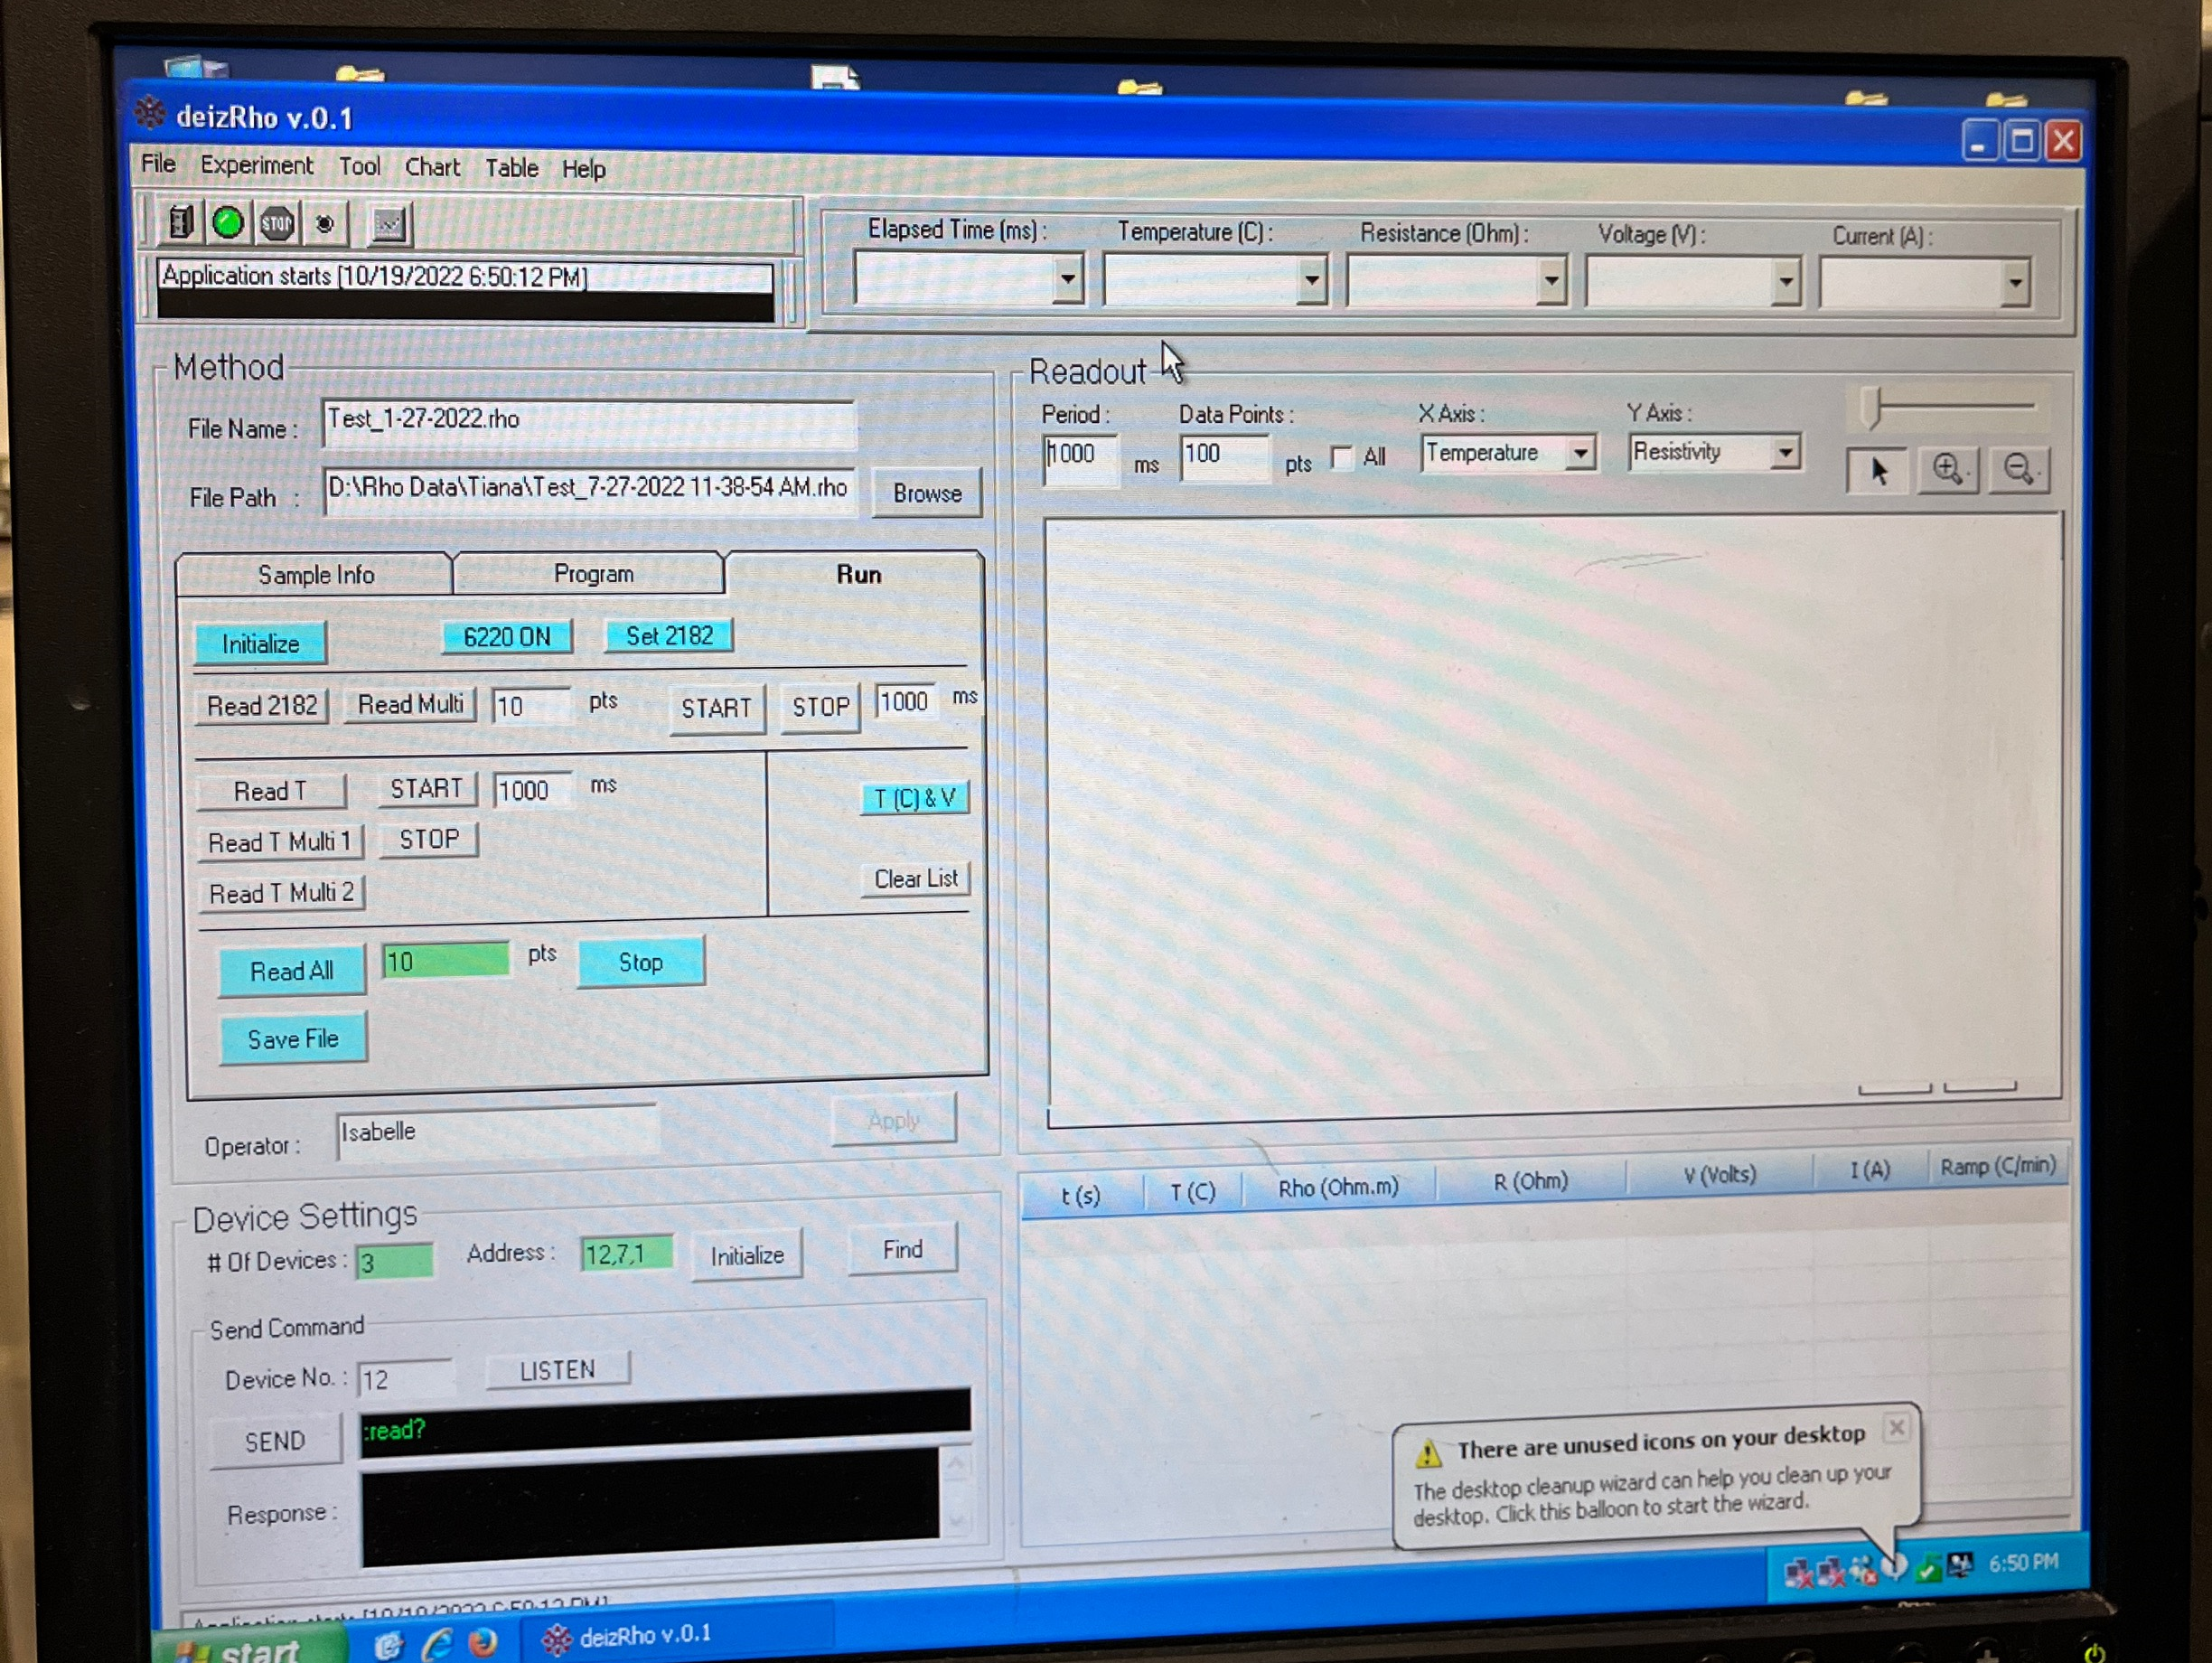
\includegraphics[scale=0.2]{app.png}}
\caption{Previous software user interface design}
\label{fig}
\end{figure}

\noindent The key elements of the existing implementation will also be included in our implementation. This is so that the application will be familiar to the user and as intuitive as possible. These elements are listed below:
\begin{itemize}
  \item Method Panel: controls which device to read data from (temperature or voltage), and which file to save the data in
  \item Device Settings Panel: used to send SCPI commands directly to a device
  \item Readout: includes graphical output and listed output of relevant values (current, voltage, resistance, etc.)
\end{itemize}

\noindent The primary differences between the existing implementation and our implementaion are the appearance of the GUI and the option of remote access. The existing implementation was developed for Windows XP whereas our implementation is developed for Windows 10, which gives it an updated look. One of the stretch goals for this project is to enable remote access to the application to be able to monitor and stop experiments remotely. The existing implementation does not have this functionality.\\


\section{Unit Testing}
In this section, the results of each unit test case is shown for each module. The module for graphical output utilizes a third party module so it will not be tested.\\

\subsection{Input Communication Module}
The table below shows the results of each unit test case in the Input Communication Module.\\
\\
\begin{tabular}{ |p{1.4cm}||p{2cm}|p{2.5cm}|p{3cm}|p{3cm}|p{1.5cm}|}
  \hline
  \multicolumn{6}{|c|}{Unit Tests for Input Communication Module} \\
  \hline
  Unit Test ID & Description & Input & Expected Output & Output & Result\\
  \hline
  UT-IC1   & Testing the getUserInput Method  &  SamplingRate : 60, SampleLength : 4; SampleWidth : 2; Filename : sample1; Name : Bob; SampleName :sample1; Date : 03/01/2023 & UserInput( SamplingRate : 60; SampleLength : 4; SampleWidth : 2; Filename : sample1; Name : bob; SampleName : sample1; Date : 03/01/2023) & UserInput( SamplingRate : 60; SampleLength : 4; SampleWidth : 2; Filename : sample1; Name : bob; SampleName : sample1; Date : 03/01/2023) & PASS \\
  \hline
  UT-IC2   & Testing the getUserInput Method &   & INVALID & INVALID  & PASS \\
  \hline
  UT-IC3   & Testing the getHardwareInput Method  &  Voltage : 5 ; Time : 10:00; Temperature : 50; Current: 1 & HardwareInput( Voltage : 5 ; Time : 10:00; Temperature : 50; Current: 1 ) & HardwareInput( Voltage : 5 ; Time : 10:00; Temperature : 50; Current: 1 ) & PASS \\
  \hline
  UT-IC4   & Testing the getHardwareInput Method &   & INVALID & INVALID  & PASS \\
  \hline
 \end{tabular}

 \pagebreak
 \subsection{Remote Access Module}
 The table below shows the results of each unit test case in the Remote Access Module.\\
\\
 \begin{tabular}{ |p{1.4cm}||p{2cm}|p{2.5cm}|p{3cm}|p{3cm}|p{1.5cm}|}
   \hline
   \multicolumn{6}{|c|}{Unit Tests for Remote Access Module} \\
   \hline
   Unit Test ID & Description & Input & Expected Output & Output & Result\\
   \hline
   UT-RA1   & Testing the connect Method  & userName: Timothy, password 12341234 & Observed connected & & FAIL \\
   \hline
   UT-RA2   & Testing the connect Method &  userName: Bob, password 12341234 & INVALID & INVALID  & PASS \\
   \hline
   UT-RA2   & Testing the connect Method &  userName: Timothy, password 56785678 & INVALID & INVALID  & PASS \\  
  \hline
  UT-RA2   & Testing the connect Method &  userName: Bob, password 56785678 & INVALID & INVALID  & PASS \\ 
   \hline
  UT-RA3   & Testing the disconnect Method &   & FALSE &   & FAIL \\ 
  \hline
  \end{tabular}

  \pagebreak
  \subsection{Current State Module}
  The table below shows the results of each unit test case in the Current State Module.\\
  \\
  \begin{tabular}{ |p{1.4cm}||p{2cm}|p{2.5cm}|p{3cm}|p{3cm}|p{1.5cm}|}
    \hline
    \multicolumn{6}{|c|}{Unit Tests for Current State Module} \\
    \hline
    Unit Test ID & Description & Input & Expected Output & Output & Result\\
    \hline
    UT-CS1   & Testing the displayUserInfo Method  & SamplingRate : 60, SampleLength : 4; SampleWidth : 2; Filename : sample1; Name : Bob; SampleName :sample1; Date : 03/01/2023 & Observed data displayed & data displayed& PASS \\
    \hline
    UT-CS2   & Testing the displayUserInfo Method  & SamplingRate : ABC, SampleLength : 4; SampleWidth : 2; Filename : sample1; Name : Bob; SampleName :sample1; Date : 03/01/2023 & INVALID & INVALID & PASS \\
    \hline
    UT-CS2   & Testing the displayUserInfo Method  & SamplingRate : -100, SampleLength : 4; SampleWidth : 2; Filename : sample1; Name : Bob; SampleName :sample1; Date : 03/01/2023 & INVALID & INVALID & PASS \\ 
   \hline
  \end{tabular}
  \newpage
  \begin{tabular}{ |p{1.4cm}||p{2cm}|p{2.5cm}|p{3cm}|p{3cm}|p{1.5cm}|}
    \hline
    \multicolumn{6}{|c|}{Unit Tests for Current State Module} \\
    \hline
   UT-CS2   & Testing the displayUserInfo Method  & SamplingRate : 60, SampleLength : ABC; SampleWidth : 2; Filename : sample1; Name : Bob; SampleName :sample1; Date : 03/01/2023 & INVALID & INVALID & PASS \\ 
    \hline
    UT-CS2   & Testing the displayUserInfo Method  & SamplingRate : 60, SampleLength : -4; SampleWidth : 2; Filename : sample1; Name : Bob; SampleName :sample1; Date : 03/01/2023 & INVALID & INVALID & PASS \\ 
    \hline
    UT-CS2   & Testing the displayUserInfo Method  & SamplingRate : 60, SampleLength : 4; SampleWidth : ABC; Filename : sample1; Name : Bob; SampleName :sample1; Date : 03/01/2023 & INVALID & INVALID & PASS \\ 
    \hline
  \end{tabular}
  \newpage
  \begin{tabular}{ |p{1.4cm}||p{2cm}|p{2.5cm}|p{3cm}|p{3cm}|p{1.5cm}|}
    \hline
    \multicolumn{6}{|c|}{Unit Tests for Current State Module} \\
    \hline
    UT-CS2   & Testing the displayUserInfo Method  & SamplingRate : 60, SampleLength : 4; SampleWidth : -2; Filename : sample1; Name : Bob; SampleName :sample1; Date : 03/01/2023 & INVALID & INVALID & PASS \\ 
    \hline
    UT-CS3   & Testing the displayHardwareState Method  & Voltage : 5 ; Time : 10:00; Temperature : 50; Current: 1 & Observed data displayed & data displayed& PASS \\
    \hline
    UT-CS4   & Testing the displayHardwareState Method  & Voltage : ABC ; Time : 10:00; Temperature : 50; Current: 1 & INVALID & INVALID& PASS \\
    \hline
    UT-CS4   & Testing the displayHardwareState Method  & Voltage : -5 ; Time : 10:00; Temperature : 50; Current: 1 & INVALID & INVALID& PASS \\
    \hline
    UT-CS4   & Testing the displayHardwareState Method  & Voltage : 5 ; Time : ABC; Temperature : 50; Current: 1 & INVALID & INVALID& PASS \\
    \hline
    UT-CS4   & Testing the displayHardwareState Method  & Voltage : 5 ; Time : -10:00; Temperature : 50; Current: 1 & INVALID & INVALID& PASS \\
    \hline
  \end{tabular}
  \newpage
  \begin{tabular}{ |p{1.4cm}||p{2cm}|p{2.5cm}|p{3cm}|p{3cm}|p{1.5cm}|}
    \hline
    \multicolumn{6}{|c|}{Unit Tests for Current State Module} \\
    \hline
    UT-CS4   & Testing the displayHardwareState Method  & Voltage : 5 ; Time : 10:00; Temperature : ABC; Current: 1 & INVALID & INVALID& PASS \\
    \hline
    UT-CS4   & Testing the displayHardwareState Method  & Voltage : 5 ; Time : 10:00; Temperature : 50; Current: ABC & INVALID & INVALID& PASS \\
    \hline
    UT-CS4   & Testing the displayHardwareState Method  & Voltage : 5 ; Time : 10:00; Temperature : 50; Current: -1 & INVALID & INVALID& PASS \\
    \hline
   \end{tabular}

\pagebreak
\subsection{Calculation Module}
The table below shows the results of each unit test case in the Calculation Module.\\
\\
\begin{tabular}{ |p{1.5cm}||p{2.5cm}|p{3cm}|p{2cm}|p{2cm}|p{1.5cm}|}
  \hline
  \multicolumn{6}{|c|}{Unit Tests for Calculation Module} \\
  \hline
  Unit Test ID & Description & Input & Expected Output & Output & Result\\
  \hline
  UT-C1   & Testing the getResistance Method  &  From HardwareInput ADT: Voltage = 5, Current = 1 & 5.000 & 5.000 & PASS \\
  \hline
  UT-C1   & Testing the getResistance Method  &  From HardwareInput ADT: Voltage = 4, Current = 0.6 & 6.667 & 6.667 & PASS \\
  \hline
  UT-C2   & Testing the getResistance Method  &  From HardwareInput ADT: Voltage = -5, Current = 1 & Invalid & Invalid & PASS \\
  \hline
  UT-C2   & Testing the getResistance Method  &  From HardwareInput ADT: Voltage = -4, Current = 0.6 & Invalid & Invalid & PASS \\
  \hline
  UT-C3   & Testing the getResistivity Method  &  Resistance = 3, Area = 2.5, Length = 2 & 3.750 & 3.750 & PASS \\
  \hline
  UT-C3   & Testing the getResistivity Method  &  Resistance = 2, Area = 2.8, Length = 1 & 5.600 & 5.600 & PASS \\
  \hline
  UT-C4   & Testing the getResistivity Method  &  Resistance = A, Area = 2.8, Length = 0 & Invalid & Invalid & PASS \\
  \hline
  UT-C4   & Testing the getResistivity Method  &  Resistance = 1, Area = 0, Length = BC & Invalid & Invalid & PASS \\
  \hline
  UT-C5  & Testing the calcResistance Method  &  Voltage = 2.6, Current = 2 & 1.300 & 1.300 & PASS \\
  \hline
  UT-C5  & Testing the calcResistance Method  &  Voltage = 3.6, Current = 2 & 1.800 & 1.800 & PASS \\
  \hline
 \end{tabular}

 \pagebreak
 \begin{tabular}{ |p{1.5cm}||p{2.5cm}|p{3cm}|p{2cm}|p{2cm}|p{1.5cm}|}
  \hline
  \multicolumn{6}{|c|}{Unit Tests for Calculation Module (Continued)} \\
  \hline
  Unit Test ID & Description & Input & Expected Output & Output & Result\\
  \hline
  UT-C6  & Testing the calcResistance Method  &  Voltage = AB, Current = 0 & Invalid & Invalid & PASS \\
  \hline
  UT-C6  & Testing the calcResistance Method  &  Voltage = 0, Current = DR & Invalid & Invalid & PASS \\
  \hline
  UT-C7  & Testing the calcResistivity Method  &  Resistance = 2, Area = 1.5, Length = 2 & 1.500 & 1.500 & PASS \\
  \hline
  UT-C7  & Testing the calcResistivity Method  &  Resistance = 1.8, Area = 1.3, Length = 1.5  & 1.560 & 1.560 & PASS \\
  \hline
  UT-C8  & Testing the calcResistivity Method  &  Resistance = AB, Area = 1, Length = 2  & Invalid & Invalid & PASS \\
  \hline
  UT-C8  & Testing the calcResistivity Method  &  Resistance = 2, Area = 2, Length = NT  & Invalid & Invalid & PASS \\
  \hline
 \end{tabular}

 \pagebreak
 \subsection{User Input Validation Module}
 The table below shows the results of each unit test case in the User Input Validation Module.\\
\\
 \begin{tabular}{ |p{1.5cm}||p{2cm}|p{2.5cm}|p{2cm}|p{2cm}|p{1.5cm}|}
  \hline
  \multicolumn{6}{|c|}{Unit Tests for User Input Validation Module} \\
  \hline
  Unit Test ID & Description & Input & Expected Output & Output & Result\\
  \hline
  UT-UI1   & Testing the getUserInput Method  &  N/A  & UserInput (SamplingRate: 60, SampleLength: 4, SampleWidth:2) & UserInput (SamplingRate: 60, SampleLength: 4, SampleWidth:2) & PASS \\
  \hline
  UT-UI2   & Testing the validateFileData Method  &  FileName: Test, Date: 03/01/2023, Name: Test & TRUE & TRUE & PASS \\
  \hline
  UT-UI2   & Testing the validateFileData Method  &  FileName: Output, Date: 03/01/2023, Name: John & TRUE & TRUE & PASS \\
  \hline
  UT-UI3   & Testing the validateFileData Method  &  FileName: Output, Date: Someday, Name: Tester & FALSE & FALSE & PASS \\
  \hline
  UT-UI3   & Testing the validateFileData Method  &  FileName: 0, Date: 03/01/2023, Name: 0 & FALSE & FALSE & PASS \\
  \hline
 \end{tabular}

 \pagebreak 

 \begin{tabular}{ |p{1.5cm}||p{2cm}|p{2.5cm}|p{2cm}|p{2cm}|p{1.5cm}|}
  \hline
  \multicolumn{6}{|c|}{Unit Tests for User Input Validation Module (Continued)} \\
  \hline
  Unit Test ID & Description & Input & Expected Output & Output & Result\\
  \hline
  UT-UI4   & Testing the validateSampleData Method  &  SamplingRate: 50, SampleLength:2, SampleWidth:5 & TRUE & TRUE & PASS \\
  \hline
  UT-UI4   & Testing the validateSampleData Method  &  SamplingRate: 60, SampleLength:1.5, SampleWidth:3 & TRUE & TRUE & PASS \\
  \hline
  UT-UI5   & Testing the validateSampleData Method  &  SamplingRate: -7, SampleLength:1.5, SampleWidth:3 & FALSE & FALSE & PASS \\
  \hline
  UT-UI5  & Testing the validateSampleData Method  &  SamplingRate: 60, SampleLength:-5, SampleWidth:3 & FALSE & FALSE & PASS \\
  \hline
 \end{tabular}

 \pagebreak
 \subsection{Hardware Input Validation Module}
 The table below shows the results of each unit test case in the Hardware Input Validation Module.\\
 \\
 \begin{tabular}{ |p{1.5cm}||p{2cm}|p{2cm}|p{3cm}|p{3cm}|p{1.5cm}|}
  \hline
  \multicolumn{6}{|c|}{Unit Tests for Hardware Input Validation Module} \\
  \hline
  Unit Test ID & Description & Input & Expected Output & Output & Result\\
  \hline
  UT-HI1   & Testing the getHardwareInput Method  &  -  & HardwareInput ( Voltage: 5, Current: 3) & HardwareInput ( Voltage: 5, Current: 3) & PASS \\
  \hline
  UT-HI2   & Testing the validateParameters Method  &  Voltage: 3.0 , Time: 5:31 PM , Current: 1.0 & TRUE & TRUE & PASS \\
  \hline
  UT-HI2   & Testing the validateFileData Method  &  Voltage: 3.2 , Time: 5:45 PM , Current: 1.2 & TRUE & TRUE & PASS \\
  \hline
  UT-HI3   & Testing the validateFileData Method  &  Voltage: 10 , Time: 5:48 PM , Current: NY & FALSE & FALSE & PASS \\
  \hline
  UT-HI3   & Testing the validateFileData Method  &  Voltage: YT , Time: 5:51 PM , Current: 0.5  & FALSE & FALSE & PASS \\
  \hline
 \end{tabular}

\subsection{Functional Requirements Testing}

\begin{table}[H]
	\centering
	\caption{Unit Tests for Functional Requirements}
	\label{my-label}
	\begin{tabular}{|p{0.85cm}|p{5cm}|p{5cm}|p{1.3cm}|}
		\hline
		\textbf{ID} & \textbf{User Action} & \textbf{Expected Result}  & \textbf{Result}\\ \hline
		UT1 & Check "Current Source" radio button & Current Source is reset & PASS \\ \hline
		UT2 & Type an integer (1) in the "Current Supply" textbox and click "Set" button & Current Supply is set to 1mA and displayed & PASS \\ \hline
		UT3 & Type an integer (10) in the "Compliance" textbox and click "Set" button & Compliance voltage is set to 10V & PASS\\ \hline
		UT4 & Click "Current ON" button & Current Source is supplying current & PASS \\ \hline
		UT5 & Click "Current OFF" button & Current Source stops supplying current & PASS \\ \hline
		UT6 & Check "Nano-Voltmeter" radio button & Nano-Voltmeter is reset & PASS \\ \hline
		UT7 & Click "Start Capture" button & Values from the voltmeter are continuously displayed on the application along with real-time calculations & PASS  \\ \hline
		UT8 & Click "Stop Capture" button & Values and calcualtions stop generating, latest batch remains visible & PASS \\ \hline
		UT9 & Current supply is set up and capture is started & Accurate calculations of resistivity are displayed continuously & PASS \\ \hline
	\end{tabular}
\end{table}

%\newpage

\begin{table}[H]
	\centering
	\begin{tabular}{|p{1cm}|p{5cm}|p{5cm}|p{1.3cm}|}
		\hline
		\textbf{ID} & \textbf{User Action} & \textbf{Expected Result}  & \textbf{Result}\\ \hline
		UT10 & System is capturing values, thermal treatment is taking place & Critical changes in resistivity are noted in the capture log & FAIL*\\ \hline
		UT11 & System is capturing values, no thermal treatment & No critical changes in resistivity are noted & PASS\\ \hline
		UT12 & Choose an "Integration Rate" of (1 PLC) from the drop-down menu & Voltmeter display shows faster reading than default & PASS \\ \hline
		UT13 & Choose an "Integration Rate" of (5 PLC) from the drop-down menu & Voltmeter display shows no change than default rate & PASS\\ \hline
		UT14 & System is capturing values, thermal treatment is taking place & Changes in resistivity-temperature slopes are noted in caputre log and displayed & FAIL* \\ \hline
		UT15 & System is capturing values, no thermal treatment & No changes in resistivity-temperature slopes are noted in caputre log or displayed & PASS \\ \hline
		UT16 & Current supply is set up and capture is started, "Stop Experiment" button is clicked on remote interface & Capture and current supply are turned off & FAIL* \\ \hline
		UT17 & Current supply is set up and capture is started, remote interface is launched but not interacted with & Capture and current supply stay on (no change) & FAIL* \\ \hline
	\end{tabular}
\end{table}

\section{Changes Due to Testing}

\noindent Based on the feedback from our Rev 0 Demo, we found that our application failed some requirements tests. The major failures were the lack of two main features: the graphical output (which still did not display real data as of Rev 0 Demo) and the ability to save output data to a chosen file. While we did not need to "test" our application to know this, we still consider these to be failed tests, as our application failed to meet requirements set out by the project supervisor. These two features have been implemented for the final demo. \\

\begin{tabular}{ |p{3cm}|p{5cm}|p{5cm}| }
  \hline
  \textbf{Test ID} & \textbf{Failure Observed} & \textbf{Change(s) Made} \\
  \hline 
  ST6 & Graph only displays dummy data & Bug with displaying real-time data was fixed \\ \hline
  ST7 & There is no method to output data to a file & File system browser and writing to output file was added \\
  \hline
 \end{tabular}


\section{Automated Testing}

\noindent We achieved automated unit testing through the use of the NUnit testing framework in Visual Studio. NUnit is one of the most popular test frameworks used for running tests on a .NET project.\\

\noindent NUnit tests are setup by first creating a new project file in Visual Studio and adding it to the solution file for your project (in our case, the application). In the new project file, a new class is created. Each unit test we want to carry out is written as a method of the test class. Since the project file for the test class is inlcuded in the same solution file as our application, we are able to call the test methods from our main application to run the tests.\\
		
\section{Trace to Requirements}
The table below shows the traceability between each non functional requirement from the SRS, and the test requirement in this report.\\
\\
\begin{tabular}{ |p{3cm}||p{4cm}|p{4cm}|p{4cm}|p{4cm}| }
  \hline
  \multicolumn{3}{|c|}{Traceability Matrix to Non Functional Requirements} \\
  \hline
  Requirement Type & Requirement(SRS) & Test Requirement \\
  \hline
  Non Functional   & NFR-U1  & NF-UT1  \\ \hline
  Non Functional   & NFR-U2  & NF-UT2  \\ \hline
  Non Functional   & NFR-U3  & NF-UT3  \\ \hline
  Non Functional   & NFR-U4  & NF-UT4  \\ \hline
  Non Functional   & NFR-U5  & NF-UT5   \\ \hline
  Non Functional   & NFR-U6  & NF-UT6  \\ \hline
  Non Functional   & NFR-P1  & NF-PT1  \\ \hline
  Non Functional   & NFR-P2  & NF-PT2  \\ \hline
  Non Functional   & NFR-P3  & NF-PT3  \\ \hline
  Non Functional   & NFR-P4  & NF-PT4  \\ \hline
  
 \end{tabular}

 The table below shows the traceability between each functional requirement from the SRS, and the test requirement in this report.\\
\\
 \begin{tabular}{ |p{3cm}||p{4cm}|p{4cm}| }
  \hline
  \multicolumn{3}{|c|}{Traceability Matrix to Functional Requirements} \\
  \hline
  Requirement Type & Requirement(SRS) & Test Requirement \\
  \hline
  Functional   & FR1  & FR-T1 \\ \hline
  Functional   & FR2  & FR-T2  \\ \hline
  Functional   & FR3  & FR-T3 \\ \hline
  Functional   & FR4  & FR-T4  \\ \hline
  Functional   & FR5  & FR-T5  \\ \hline
  Functional   & FR6  & FR-T6 \\ \hline
  
 \end{tabular}

\begin{table}[H]
	\centering
	\caption{Requirements Traceability}
	\label{my-label}
	\begin{tabular}{|c|c|c|c|}
		\hline
		\textbf{System Test} & \textbf{Unit Tests} & \textbf{Requirement} & \textbf{Plan} \\ \hline
		ST1 & UT1 — UT9 & FR1 &FR-T1 \\ \hline
		ST2 & UT10, UT11 & FR2 &FR-T2\\ \hline
		ST3 & UT12, UT13 & FR3 &FR-T3\\ \hline
		ST4 & UT14, UT15 & FR4 &FR-T4\\ \hline
		ST5 & UT16, UT17 & FR5 &FR-T5\\ \hline
		ST6 &  & FR6 &FR-T6\\ \hline
		ST7 &  & FR7 &FR-T7\\ \hline
	\end{tabular}
\end{table}
		
\pagebreak
\section{Trace to Modules}		
The table below shows the traceability between each module, and its respective unit tests in this report.\\
\\
\begin{tabular}{ |p{5cm}||p{5cm}| }
  \hline
  \multicolumn{2}{|c|}{Traceability Matrix to Modules} \\
  \hline
  Module & Unit Tests \\
  \hline
  Input Communication   & UT-IC1, UT-IC2, UT-IC3, UT-IC4  \\ \hline
  Remote Access   & UT-RA1, UT-RA2, UT-RA3   \\ \hline
  Current State   & UT-CS1, UT-CS2, UT-CS3, UT-CS4   \\ \hline
  File Output   & -  \\ \hline
  Calculation   & UT-C1, UT-C2, UT-C3, UT-C4,UT-C5, UT-C6, UT-C7, UT-C8   \\ \hline
  User Input Validation  & UT-UI1, UT-UI2, UT-UI3, UT-UI4, UT-UI5   \\ \hline
  Hardware Input Validation  & UT-HI1, UT-HI2, UT-HI3  \\ \hline
  
 \end{tabular}

\bibliographystyle{plainnat}
% \bibliography{../../refs/References}

\newpage{}
\section*{Appendix --- Reflection}

The information in this section will be used to evaluate the team members on the
graduate attribute of Reflection.  Please answer the following question:

\begin{enumerate}
  \item In what ways was the Verification and Validation (VnV) Plan different
  from the activities that were actually conducted for VnV?  If there were
  differences, what changes required the modification in the plan?  Why did
  these changes occur?  Would you be able to anticipate these changes in future projects?  If there weren't any differences, how was your team able to clearly predict a feasible amount of effort and the right tasks needed to build the evidence that demonstrates the required quality?  (It is expected that most teams will have had to deviate from their original VnV Plan.)
\end{enumerate}

\indent There were several differences between what we had planned for VnV and what we ended up carrying out. When completing the initial revision of VnV plan, we had not yet completed the Design documents (MG, MIS, System Design) and so we did not have a plan for unit/module testing, only for system testing. Our initial VnV plan included three main sections: SRS Verification, Design Verification, and Implementation Verification.\\

\indent For SRS Verification, we planned to meet every two weeks to discuss potential updates to the SRS doc. While we continued to meet frequently (weekly or bi-weekly), our team focussed instead on the next deliverable rather than revisiting old documents during meetings. Because of this, our SRS was not continually being updated during the project. This change occurred mainly due to time constraints, as we faced some technical issues leading up to the first demo which took priority over other tasks. In hindsight, frequently revisiting and updating the SRS certainly would have created less work for us in the long run. For future projects, though we can't predict any exact technical issues that would set us back on time, we should be able to anticipate issues arising which cause delays. We should have a plan to stay on schedule despite such issues. \\

\indent  For Design Verification, we planned to use the MIS checklist to ensure that requirements in the SRS are met and hazards in the Hazard Analysis are covered. Our team followed the MIS checklist when testing. We also planned to use feedback from the course instructor, teaching assistants, classmates, and our project supervisor. There were not many changes made in this section of the plan, except that our team decided to focus primarily on feedback from Dr. Zurob, as he is the end-user of the application. \\

\indent For Implementation Verification, we planned to used GitHub issues and pull requests to maintain our code base. Any pull request made to the main branch requires at least two other team members to review and approve. We did not make any major changes to our Implementation Verification plan. 
\end{document}